\chapter{Research Background}

%\todo[inline]{Talk about what is important for this thesis}
%\todo[inline]{Check for overlaps with text in chapters 4,5,6,7,8.}

This dissertation is in the intersection between process mining and mining software repositories, respectively belonging to the broader contexts of \gls{bpm} and software development process. This chapter, hierarchically delves into the details of these fields as follows. \Cref{sec:software-development} gives an introduction on the main concepts of the software development process, elaborating on methodologies and repositories in which the data is stored.
\Cref{sec:bpa} provides an overview on \gls{bpm} and introduces the \gls{bpm} lifecycle, and describes the specific area of process mining along with its requirements and limitations when analysing software. \Cref{sec:ch2-summary} summarizes they key concepts presented in this chapter. 
%\Cref{sec:visualization} provides an overview on the area of software visualization. 

%\Cref{sec:project-oriented} illustrates a class of processes which belong to the intersection between software development and business process. 
%The remaining sections further introduce research streams upon which to draw solutions for data-driven analyses of software development processes. \Cref{sec:text-mining} shortly describes the area of text mining, used for extracting knowledge from unstructured data. Finally, \Cref{sec:summary-of-relevant-techniques} summarizes these solutions. 
 

%This chapter is concerned with data-driven approaches used in literature to \emph{solutions}, which help tackling the problem of monitoring software development. Four disciplines provide the necessary theoretical and practical knowledge upon which this thesis is built. Thus, this chapter presents these four disciplines as follows. \Cref{sec:process-mining} briefly describes the area of process mining. \Cref{sec:msr} describes contributions from the area of mining software repositories. \Cref{sec:visualization} provides an overview on the area of software visualization. \Cref{sec:text-mining} shortly describes the area of text mining, used for extracting knowledge from unstructured data. Finally, \Cref{sec:summary-of-relevant-techniques} summarizes these solutions. 

\section{Software Development Process}
\label{sec:software-development}


Software is the set of instructions in the form of programs to govern the computer system and to process the hardware components. To produce a software product, a set of systematic activities are undertaken. This set is called a \emph{software development process}. 
Good software should deliver the required functionality and performance to the user and should be maintainable, dependable and usable \citep{sommerville2011software}. All aspects of software production are managed by the discipline of \emph{software engineering}. 
Key activities of software engineering can be grouped into four macro phases: 
\begin{inparaenum}[\itshape i)]
	\item Requirements, 
	\item Design and Implementation, 
	\item Validation and 
	\item Evolution. 
\end{inparaenum}


Generally accepted knowledge about the software engineering discipline is defined in the \gls{swebok} \citep{borque2014guide}. In particular, the aforementioned phases are defined as follows. 
The requirements phase is concerned with the elicitation, analysis and specification of the what is need for the software product to fulfil desired goals. Goals can be functional requirements (i.e., how the software must work, given its inputs and outputs),  non-functional requirements (i.e., portability, re-usability, flexibility, performance, etc), and domain requirements (i.e., other aspects imposed by the specific domain).

Design and Implementation are respectively the phases in which a general architecture of the software is defined and the phase in which the software is developed. Design includes that definition of what the software should do at different levels of abstraction: interface, system, and detailed design. Interface design is concerned with the interaction between software and surrounding environment. System design defines the major software components, their interfaces and the interaction among them. Detailed design delves into the details of the aforementioned systems and defines their internal properties such as the specific algorithms or data structures. Finally, software implementation is the actual task of programming (i.e., writing the code, bug fixing, testing, debugging, documenting, etc).

Software Validation is the sub-process in which the produces software artifact is tested against the business requirements and end user needs. Software evolution is the process that concerns both the maintenance and the update of the software product. 

%It was in the late 1960s when many software projects failed.
%Many software became over budget. Output was an unreliable software which is expensive to maintain.
%Larger software was difficult and quite expensive to maintain.
%Lots of software not able to satisfy the growing requirements of the customer.
%Complexities of software projects increased whenever its hardware capability increased.
%Demand for new software increased faster compared with the ability to generate new software.


\begin{figure}
	\centering
	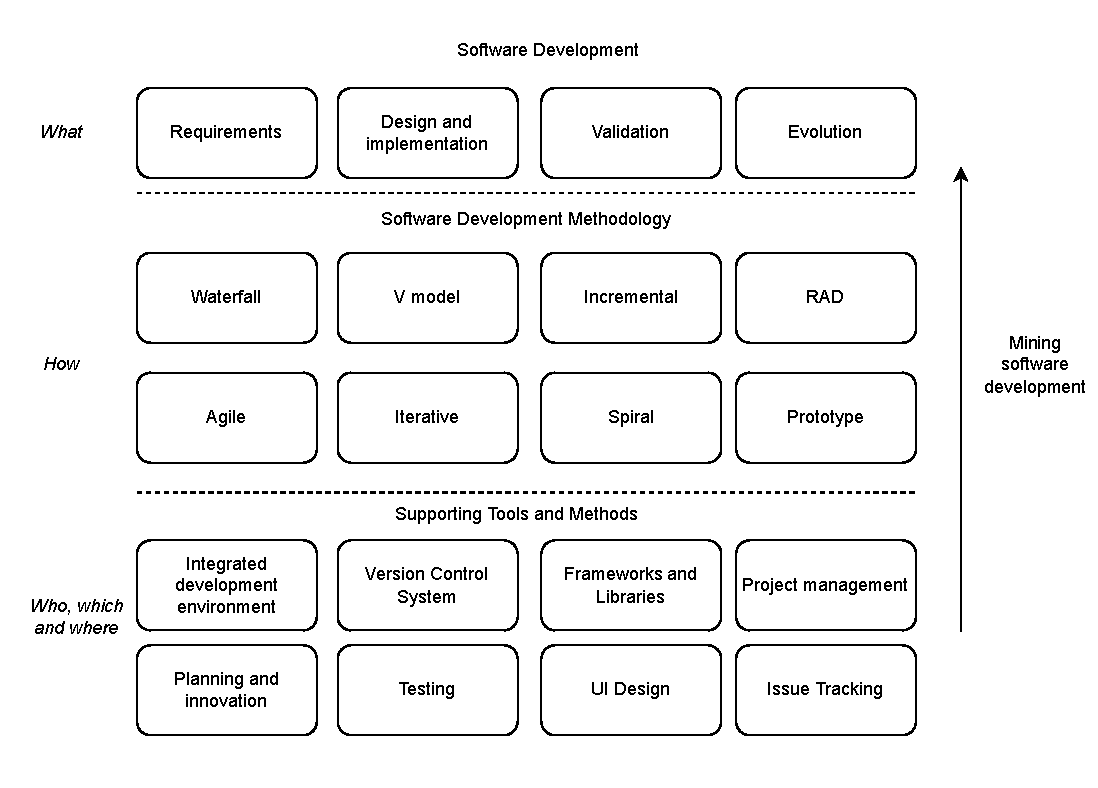
\includegraphics[width=\linewidth]{figures/SoftwareBigPic2}
	\caption{Software production as an engineering discipline}
	\label{fig:soft-eng}
\end{figure}


%\subsection{Overview on Software Development}


\Cref{fig:soft-eng} gives an overview on software development (i.e., the practice of diving the creation of a software artifact into smaller steps). It is possible to observe the overall practice of software development under three main dimensions: 
\begin{inparaenum}[\itshape i)]
	\item the type of activities or processes involved (i.e., \emph{what} work is being done);
	\item the methodology used (i.e., \emph{how} the work is conducted); and 
	\item the supporting tools and frameworks (i.e., \emph{which} software facilities developed by \emph{whom} and stored \emph{where} are being used). 
\end{inparaenum}


The software development dimension captures and defines at different level of detail, all the activities that concern software development. Typical activities here are the ones defined in \gls{swebok} \citep{borque2014guide} such as Requirements, Design, Implementation, Validation, and Evolution. 

Naturally, there are many possible approaches to software production by changing the way, time, and frequency these activities and in how many smaller steps they are performed.
The totality of the steps is also called \gls{sdlc}.  There are many existing methodologies, each with an specific life-cycle.
The Software Development Methodology phase is concerned with what \gls{sdlc} was followed. Typical methodologies include Waterfall, V-Model, Incremental, \gls{rad}, Agile, Iterative,  Spiral, and Prototype.
%The final goal is to create or improve an existing piece of software. Each step typically defines specifications about the input and output. The totality of the steps is also called software development life cycle. There are many existing methodologies, each with an specific life-cycle.
%Popular methodologies are agile, waterfall, spiral, rapid application development and extreme programming.



Finally, as the complexity of produced software grows (i.e., more features, bigger codebase, more modules, higher integration), so do the number of tools used to support the software process. Under the supporting tools and methods dimension fall all existing hardware, software and management techniques that are used as scaffold to develop more advanced software pieces. Key elements in this dimension are version control systems and the repositories on which the data is stored. Other examples of supporting tools and methods include \glspl{ide}, frameworks and libraries, project management software, issue tracker, etc. Details about software development methodologies, and supporting tools and methods follow in the next sections.


%The software development process is a specific kind of process. Differently from standard business processes, it is run without referring to a process model (e.g., BPMN, Petri net). A common trait of both software development and business is the fact that they both describe and endeavor to organize work in such a way that should be measured and hence monitored and improved. Therefore, both areas rely on methods for managing their processes. Popular methodologies in software development are Waterfall, Spiral, and Agile. Agile methods further refine into branches such as Scrum and Kanban. In order to measure the effectiveness of these methodologies, we can analyze the underlying trace data that is generated in the various steps. In the following, we further elaborate on software development methodologies and the software repositories used to keep track of the development process. 





\subsection{Software Development Methodologies}

A software development methodology is a process or a series of processes used in software development \citep{elliott2004global}. It generally takes the form of defined phases \citep{kruchten2004rational} such as design, testing, etc. It is used to describe the life-cycle of a piece of software (how it came to be and how it will evolve further). It can be used for communication (i.e., how information is passed between collaborators and when).  \Cref{fig:soft-eng} defines some popular software development methodologies. Even though in practice it is common to use adaptations or combinations of these methodologies, the most popular characterization is as follows \begin{inparaenum} [\itshape i)]
	\item Waterfall, 
	\item V model,
	\item Incremental model,
	\item \gls{rad} model,
	\item Spiral model,
	\item Agile model,
	\item Iterative model, and
	\item Prototype model.
\end{inparaenum} 

The waterfall model \citep{DBLP:conf/icse/BellT76} breaks down the software development activities into sequential steps, typically Requirements, 
Software design,  Implementation, Testing, Integration, Deployment,  and Maintenance. Each depends on the outcome of the previous step. The spirit of waterfall is that the process keeps flowing forward (similar to the flow of water in a waterfall) without ever going back to a previous phase. Waterfalls provides advantages when it comes to project control 
and proper documentation. However, its long time to deliver a finite product makes this \gls{sdlc} model not suitable for long lasting projects or project in which requirements may change often \citep{DBLP:conf/profes/PetersenWB09}. 

The V-Model \citep{ForsbergMooz1992} is considered as an extension of Waterfall. In the case of the V-Model the development process is done sequentially until the development phase, after which it runs backwards across each phase and performs testing. It is also known as Verification and Validation model. That is, there is an associated testing to each development step. A sequence in the process is as follows:  \textit{Requirement Analysis} (1) $\rightarrow$ \textit{System Design} (2) $\rightarrow$ \textit{Architecture Design} (3) $\rightarrow$ \textit{Module Design} (4) $\rightarrow$ \textit{Coding} (5) $\rightarrow$ \textit{Unit Testing} (validate  4) $\rightarrow$ \textit{Integration Testing} (validate 3) $\rightarrow$ \textit{System Testing} (validate 2) $\rightarrow$ \textit{Acceptance Testing} (validate 1). While the V-Model is easy to learn and use, and enables a priori planning of the tests to be executed for each phase, it's limitations remain the same as Waterfall (i.e., rigid model not suitable to changing requirements and fast delivery) \citep{marick1999new}.

The incremental model \citep{pressman2005software} is a variation of Waterfall in which the requirements are broken down into multiple modules. Each of module is addressed performing all the \gls{sdlc} steps: requirement analysis, design, code and test. The release of each module is an increment (i.e., addresses more requirements and contains more features). However, the software is deployed already after the first increment has been delivered. This speeds up the generation of a first core product which can be used by the customer. Clients can then analyse and participate in planning of the next increment. Critics to this model concern the long duration of the overall project, the low flexibility of each iteration phase, and the fact that possible architectural limitations only emerge at a later stage when the complexity grows \citep{mishra2013comparative}.

The \Glsfirst{rad} model \citep{martin1991rapid} is a methodology that puts more emphasis on the rapid construction of prototypes rather than upfront planning. It is organized around four phases: Requirements planning, User design, construction and cutover. Requirements planning includes both planning and analysis of the requirements. User design has user communicate with developers in a continuos and interactive fashion until the model meets their needs. Construction is concerned with the programming task, although users can still contribute with suggestions of changes. Cutover phase put together the final activities of traditional \glspl{sdlc} (i.e., delivery, deployment, maintenance, user training, etc.). Advantages of \gls{rad} are its short development cycle, and, thanks to user involvement, risk control and better quality.
Disadvantages of \gls{rad} include ineffective communication, confusion of roles and responsibilities and less project control as users can interact directly with developers rather than business analysts \citep{gerber2007practical}.

The spiral model \citep{DBLP:journals/computer/Boehm88} combines aspects of traditional \glspl{sdlc} and \gls{rad} by iterating over various phases a number of times. In this way this model mitigates the risk by delivering early and planning the next release after a cycle is complete. However, this development model turns not be viable for smaller projects due to high costs and the high expertise needed to assess risk analyses after each phase \citep{sarker2015survey}.

The agile model \citep{beck2001manifesto} is an umbrella term for several methodologies like Scrum, Kanban, Lean, etc. Agile approaches help people involved in software development by empowering the teams to quickly react to changes as requirements evolve. Advantages of agile include customer satisfaction due to quick releases and quick responses to a change. As well, agile puts an emphases on people rather than processes, giving the participants better means of communication and interaction. Disadvantages of agile emerge when projects become more complex, especially due to less focus on design and documentation. Another disadvantage is that, although being empowered, only expert programmers are capable of making the right decisions as the project grows more complex \citep{DBLP:journals/jss/DingsoyrNBM12}.

The iterative model \citep{goldberg1995succeeding} applies the philosophy of starting small and iteratively increasing the set of features. In this sense, the approach is similar to the incremental methodology. However, differently from the incremental approach, requirements are not worked on in an isolated fashion but rather categorized and sorted by priority. Advantages of iterative development include early delivery, risk mitigation and adaptability to changes. Disadvantages include the need for a priori knowledge of all the requirements, hard to make new developed parts work together as the project grows more complex \citep{benediktsson2003cocomo}.


The prototype model \citep{pressman2005software} starts with building a toy example before carrying out the actual development. This toy example (prototype) is used to test the capabilities and reason about the software to-be. In this way, customer requirements and expectations can better align with the teams skills and capabilities. Other advantages include early support and early identification of errors. Disadvantages of prototyping include risk of unstable prototype becoming part of the final product, time-consuming development of prototypes and difficult project planning \citep{DBLP:conf/cicsyn/OsmaniAI14}. 

Independently of the methodology used, modern software development increasingly relies on tool and method support. For example, in order to build a new piece of software, libraries containing existing solutions, \glspl{ide} helping with structuring the codebase, and repositories offering reliable options for storing and tracking the work, enable development teams to deliver software of better quality quicker and cheaper. All these tools generate event logs which are stored in \emph{software repositories} for posthumous analysis. Next section provides a background on software repositories. 

%\todoinline{Cut the following?}
%
%
%
%
%
%
%Existing research shows that making explicit the knowledge defined by \glspl{sdm} improves productivity of software development enterprises and quality of the developed software. This is achieved by increasing enterprises’ ability to transfer knowledge between employees, systematically manage software development process, etc. \citep{avison2003information,DBLP:journals/iam/Fitzgerald98,hovelja2015exploring,DBLP:journals/tse/RiemenschneiderHD02}. However, it is not enough that an enterprise only describes its SDM in a document; the developers need to use it consistently in their everyday work. The use of SDM was often a topic of research in the last decades, since SDM adoption among software developers was relatively low and the developers often preferred different ad hoc approaches \citep{DBLP:journals/software/Aaen03,DBLP:journals/isj/Fitzgerald96,DBLP:journals/iam/HuismanI06}. 
%
%The use of SDMs in enterprises can be analyzed with the help of different existing approaches (\citealp{DBLP:journals/imds/Aboelmaged10,venkatesh2000theoretical,DBLP:journals/behaviourIT/WangLH13}). One of the grounding theories in the field of SDM evaluation is diffusion of innovations theory \citep{DBLP:books/daglib/0012785} according to which SDM is considered as innovation that developers adopt \citep{DBLP:journals/iam/Gallivan03,DBLP:journals/infsof/GreenHC05,DBLP:conf/caise/IivariH01}. To obtain information about the studied SDM and/or its elements the aforementioned studies focused on perceptions of different stakeholders, namely developers, managers, users, etc. to measure characteristics like level of use, assimilation, social and technical suitability, developer satisfaction and impact on performance \citep{atkinson1999project,cooper1990information,DBLP:books/daglib/0012785,DBLP:journals/infsof/VavpoticB09,DBLP:journals/comsis/VavpoticH12}. Even better insight into SDM and/or its elements can be gained by comparing the perceptions of different stakeholders regarding the same SDM and/or its element \citep{hovelja2015exploring}. 
%
%Another important theoretical development in the field was that SDM should be studied on the level of its constituent elements like activities, tools, roles, produced documents, etc. and not only as a whole. This improved the understanding of suitability of studied SDM elements for a certain development team and enabled comparison between the studied SDM elements. Thus, allowing enterprises to better pinpoint problematic elements of SDM, prepare focused improvements and examine the link between a specific SDM element and overall project success \citep{atkinson1999project,hovelja2015exploring}. Such development is in line with findings in the field of situational method engineering \citep{DBLP:journals/ejis/KarlssonA09,DBLP:conf/caise/RalyteDR03} that constructs a custom SDM from those SDM elements that fit with characteristics of certain development team and other situational factors (internal and external enterprise’s environment). 
%
%Another potential source of information regarding development process emerged in recent years with widespread use of tools that support software development activities like issue tracking, requirements management, test management etc. Such tools store valuable data about actual execution of the development process and give us additional information about SDM and its elements thus importantly complementing stakeholder perceptions \citep{DBLP:journals/ese/ChoetkiertikulD17,DBLP:conf/msr/MantylaADGO16,DBLP:conf/msr/OrtuMDTTMA16,DBLP:conf/icse/OrtuDKM15}. 



\subsection{Software Repositories}
\label{sec:software-repositories}

A software repository is a location that stores information about software \citep{oinas1999two,yamada2015classification} in a way that is centrally accessible and available for reuse \citep{DBLP:conf/sigsoft/MarcusM10}. Generally, software repositories serve the purposes of enabling \citep{DBLP:conf/itqm/SrinivasRR14} and keeping track of the collaboration among participants in a sotware project. Data stored in a repository include source code, documentation, libraries, models and other digital artifacts \citep{li2010measurement,DBLP:journals/infsof/SunLLLL15} that support the software development. Examples of software repositories are Maven\footnote{https://maven.apache.org} for Java source code and documentation, CRAN\footnote{https://cran.r-project.org} for R libraries, CTAN\footnote{https://ctan.org} for LaTeX, etc. 

Typically, interaction with a repository is handled by a repository or package manager (e.g., npm\footnote{www.npmjs.com}, PyPI\footnote{https://pypi.org}) or a platform (e.g., GitHub\footnote{https://github.com}). 
Data handled by these kind of software – especially considering platforms like GitHub – is rich. It includes both structured (e.g., remote databases, distributed spreadsheets) and unstructured information (e.g., forums, software review tools) \citep{DBLP:books/el/16/Bacchelli16,DBLP:conf/wcre/Bavota16}. More specifically,  structured data are generated by systems according to a preset schema. For example, the system may always record the amount of change to a file along with the version number and the user who last changed it. The purpose of these kind of data is to be processed by machines. Conversely, unstructured data are pieces of information that are used by developers to communicate. Examples of unstructured data are posts on forums, comments, code-reviews and emails. 

Repository managers or platforms rely on a variety of software facilities. A key type of system here is the so-called \gls{scm}, which allows to systematically organize and control the changes during the software development life-cycle \citep{DBLP:conf/icse/Estublier00}. \Gls{scm} relies on software such a \glsfirst{vcs} to keep track of the evolution of files. Notable \glspl{vcs} include Subversion\footnote{https://subversion.apache.org} and git\footnote{https://git-scm.com} \citep{torvalds2010git}. Tracking its changes, helps to both continuous integration and to create traces which can later on be analysed for compliance with norms and regulations that may require some evidence of the actions being performed in the organization.

Not all the data from software are stored in one single repository \citep{DBLP:journals/ese/KalliamvakouGBS16}. For instance, to manage the tasks of developers, software repositories may adopt an  \glsfirst{its}  \citep{DBLP:conf/cscw/BertramVGW10}. Popular \gls{its} include Jira\footnote{https://www.atlassian.com/software/jira}, Bugzilla\footnote{https://www.bugzilla.org}, Micosoft Dynamics CRM\footnote{http://dynamics.microsoft.com}, Trello\footnote{http://trello.com}, etc.  Thus, in order to gain a more complete understanding, integration of more repositories is considered. This implies that analyses of software repositories often deals with large volume of data \citep{DBLP:journals/tosem/0001NRN15,DBLP:journals/jossw/Boettiger18,DBLP:conf/wcre/BoldiPVZ20}. Typical dataset that are integrated usually combine \gls{its} and \gls{vcs} (cf. \Cref{fig:big-picture-sd}).  

To access trace data contained in repositories, a number of approaches are available \citep{Voinea2006b,DBLP:conf/icse/GousiosS17,DBLP:conf/icse/OrtuDKM15,DBLP:conf/msr/PonzanelliBPOL14}. Such technique include algorithms to access unstructured information from forums such as from the StackOverflow\footnote{stackoverflow.com} \citep{DBLP:journals/spe/HuPZXGY20}, full text search and visualisation of metrics of a software repository \citep{DBLP:conf/vissoft/FeinerA18}, and various data collection and query initiatives such as GHTorrent \citep{DBLP:conf/msr/GousiosS12}. Next section describes how these trace data are used for mining relevant information about the software process. 

%We focus on project mining motivated by a real case scenario in the scope of the SHAPE research project\footnote{\url{http://ai.wu.ac.at/shape-project/}}.
%The data log is provided by a Version Control Systems (VCS) whose information is not subdivided into traces related to process instances but consists of a hierarchy of work streams associated with individual files being added, modified or deleted in a subversion repository.



\subsection{Mining Software Repositories}
\label{sec:msr}

In literature, mining software repositories refers to the area of software engineering that applies machine learning algorithms to data from software with the goal of extracting knowledge \citep{DBLP:journals/smr/KagdiCM07,hassan2008road}. This area is used as the base for providing techniques and algorithms as solutions to engineering problems. Such problems typically revolve around questions aimed at understanding various performance \citep{Chen2016} and functionality issues \citep{Farias2016} with the software at several stages. Examples of knowledge are related to the problems \emph{where-to-log} \citep{DBLP:conf/msr/CandidoHAD21}, \emph{who-did-what} \citep{DBLP:conf/msr/YoungCMTHB21}, \emph{what-does-this-change-mean} \citep{DBLP:conf/iwpc/FluriG06}, \emph{who-can-work-on-this-bug} \citep{DBLP:conf/iwpc/KagdiP09}, etc. 


The main focus of research on mining software repositories has been on applying machine learning to discover patterns that may be used for improving the software process. \cite{DBLP:journals/smr/KagdiCM07} provided a taxonomy of approaches used in the area. According to their study, evolution of software was a key topic in the literature. More specifically, the field's focus has been on studying change and evolution, defect classification and analysis, comparing versions of the source code, reusability, development process, contribution analysis and various metrics. More recent studies \citep{DBLP:journals/pai/Guemes-PenaNSR18} confirm the focus on evolution, listing topics such as software degradation, dependencies between co-changes, bug prediction and causes, interaction between developers, software methodologies, and various aspects of software development.


From the point of view of which this thesis is concerned (i.e., process insights on software development), all various approaches can be categorized into two main groups: mining approaches and visualisation . 

Mining approaches provide various metrics and patterns that emerge from the raw data. They can be further divided into two sub-categories depending whether they work with structured or unstructured data. Approaches that work with structured data typically gives as output coupling patterns \citep{DBLP:conf/msr/SouzaM13,DBLP:journals/smr/KirbasCHCBSB17,DBLP:journals/ese/WenNLB22}, change classification \citep{kaur2018gcc,DBLP:journals/ese/HerzigJZ16}, code quality issues \citep{DBLP:conf/msr/KieferBT07,DBLP:conf/msr/ChenTNH12,DBLP:conf/icse/WangLT16}, and various software metrics \citep{DBLP:conf/icst/ZaidmanRDD08,DBLP:conf/icse/Thomas11,DBLP:conf/scam/SokolAG13}. Approaches that work with unstructured data typically apply \gls{nlp} to the information retrieved from forums such Stackoverflow \citep{DBLP:conf/msr/PonzanelliBPOL14}, code-review comments \citep{DBLP:conf/msr/OmranT17}, and other textual information contained in the repositories \citep{DBLP:journals/ese/BaruaTH14,DBLP:journals/jss/YanFZYXK16}. The final output in both cases is about producing quantitative analysis to uncover relations or patterns from trace data.

Visualisation approaches aim at taming the high amount of information contained in repositories by providing visual aids to navigate through it. Such navigation is rendered using various representations \citep{DBLP:journals/scp/TorresGSP16}. Notable representations here are software as cities \cite{DBLP:conf/vissoft/WettelL07} , graph-based visualisations \cite{DBLP:conf/icse/BhattacharyaINF12} and various charts \cite{DAmbros2009,DBLP:conf/msr/BirdGDGS06}. In this class fall also various attempts to apply process mining \citep{rubin2014process, DBLP:conf/indiaSE/GuptaS14,DBLP:conf/wecwis/MarquesSF18,DBLP:conf/bpm/JookenCJ19}. 

%Software visualisation techniques include
%
%- HPI visual software analytics 
%- Software as cities
%- Graph visualisations (e.g., social network analyses, static and dynamic graphs, )
%- Plots and charts (Dashboards)
%- Kanban/Project management KPI visualisations

%Visualizing co-change information with the evolution radar \citep{DAmbros2009}
% 
%Most of the methods are quantitative. However there are also a number of empirical studies \citep{DBLP:journals/ese/KalliamvakouGBS16,dehghan2017predicting} 

Relevant topics and techniques for this dissertation are those which work with version control, that is, historical trace data about the evolution of artifacts. This thesis falls into the category of works which try to bridge process mining with mining software repositories. 
Especially, the techniques developed in this thesis are inspired from the approaches to extract information from repositories \citep{DBLP:conf/msr/GousiosS12,DBLP:journals/ese/VasilescuSGM14} and visualisation approaches \citep{DAmbros2009} as well as approaches that explicitly target business processes \citep{DBLP:conf/csmr/PoncinSB11,DBLP:conf/oopsla/PoncinSB11} in order to develop new applications targetted at managers. 


%\section{Software Visualization}
%\label{sec:visualization}
%

%\section{Project-Oriented Business Process}
%\label{sec:project-oriented}

%Project-oriented business processes are a category of business processes which have the following characteristics. 
%
%They are usually one shot. When run twice, the second instance differs from the first. 
%
%These kind of processes have specific requirements for monitoring. 
%
%These processes are suited to describe plans. These plans can regard for example, the delivery of a software systems at a specified time and under specific restrictions of budget. 


%Business process management plays an important role for improving the performance and compliance of various types of processes. In practice, many processes are executed with clear guidelines and regulatory rules, but without an explicit centralized control imposed by a process engine. In particular, it is often important to exactly know when which work was done. This is, for instance, the case for complex engineering processes in which different parties are involved. We refer to this class of processes as project-oriented business processes.
%
%Such project-oriented business processes are difficult to control due to the lack of a centralized process engine. However, there are various unstructured pieces of information available to analyze and monitor their progress. One type of data that are often available these processes is event data from version control systems (VCS). While process mining techniques provide a useful perspective on how such event data can be analyzed, they do not produce output that is readily organized according to the project orientation of these processes.
%
%In this thesis, we define formal concepts for capturing project-oriented processes. These concepts provide the foundation for us to develop an automatic discovery technique which we refer to as \emph{project mining}. The output of our project mining algorithm is organized according to the specific structure typically encountered in project-oriented business processes. With this work, we extend the field of process mining towards the coverage of this specific type of business process.

%The class of processes that we discuss in this section are long-term engineering projects. These processes have specific requirements for monitoring. First, they are executed only once according to the specific needs of a particular project, and only partially according to recurring process descriptions. Second, they involve various actors that typically document their work in a semi-structured way using text and tables. Third, work in the project is usually subject to constraints regarding the start and end and the temporal order. Fourth, there is typically no process engine controlling the execution. Fifth, even though these limitations in terms of traceability exist, there are usually strong requirements in terms of tracking when which work was conducted.
%
%%Unlike other types of business processes, the processes we consider here
%%representing such projects are specifically tailored to customer needs the specific needs of the project, and there is
%
%In line with these observations, a \textit{project-oriented business process} can be defined as an ad-hoc plan that specifies the tasks to be performed within a limited period of time and with a limited set of resources for achieving a specific goal. Unlike repetitive business processes for which notations such as \gls{bpmn}~\citep{bpmn2_stable} or \gls{epc}~\citep{vanderaalst_formalization_1999} are commonly used, project-oriented business processes may be properly represented with \gls{pert} or GANTT models. The concept is illustrated in Fig.~\ref{fig:bpm2015problem}.
%
%
%\begin{figure}[htbp!]
%	\centering
%	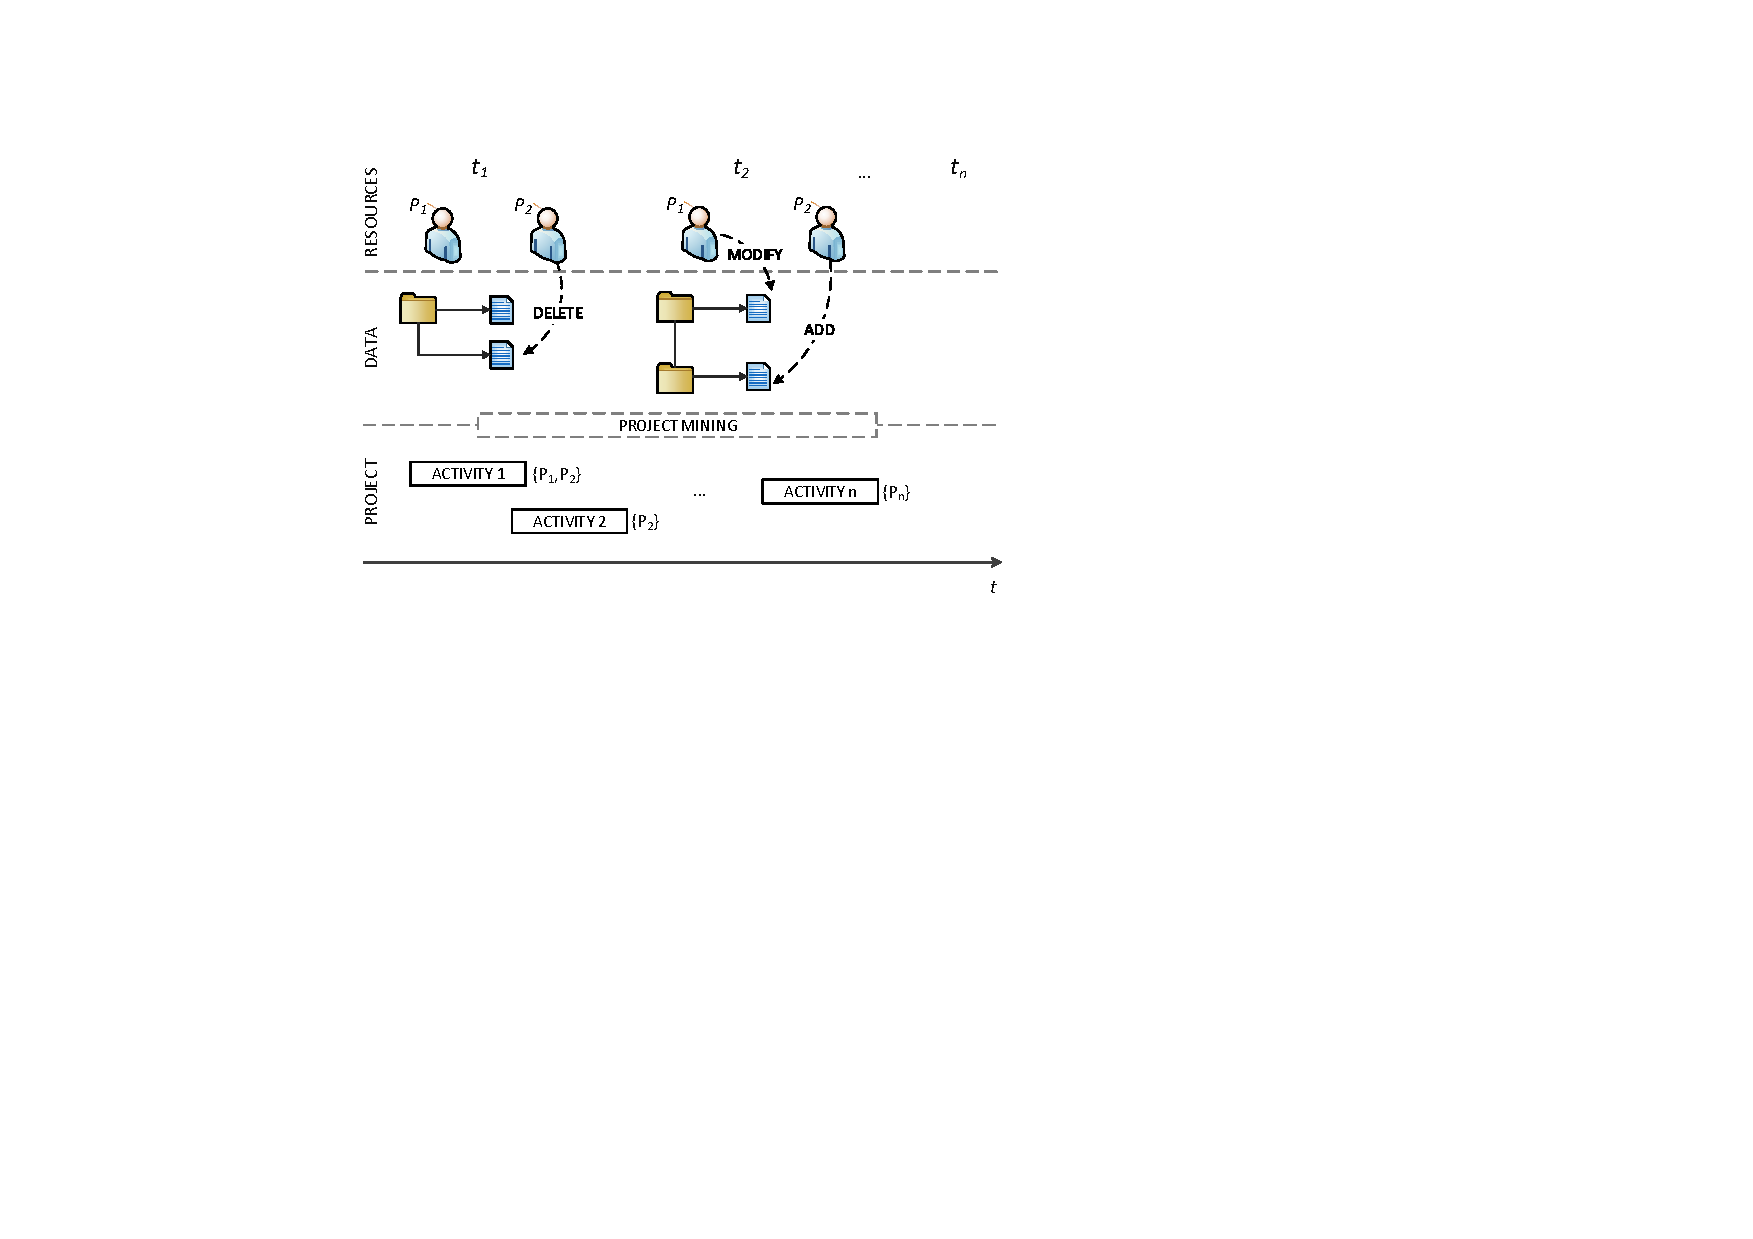
\includegraphics[width=.8\textwidth]{bpm2015/imgs/ProjectMining.pdf}
%	\caption{Gap between User-Generated Artifacts and Project-Activities}
%	\label{fig:bpm2015problem}
%\end{figure}
%
%
%Software development processes can also be seen as project-oriented business processes. They share some common characteristics. First, they involve various resources with different roles. In the simplest case, we can distinguish \emph{project managers} and \emph{project participants}. Project managers are responsible for managing the development process and supervising the work of the project participants, who in turn are responsible for specific work tasks. Second, such processes are usually subject to constraints in terms of cost, time and quality, which is mostly associated with the performance of each of the work tasks. Third, the project participants work on a plethora of artifacts, which are logically organized in a hierarchical structure, with complex interdependencies among them.
%Given these characteristics, it is the goal of the project manager to organize the software development process in such a way that the work on different files and tasks reflects the complex interdependencies, the constraints and the available participants. Therefore, it is important for the manager to understand the \emph{work history} of the process in order to monitor the progress systematically.

%project specifies the tasks to be performed considering a hierarchy of files, within a limited period of time, and with a limited set of project participants, for achieving a specific goal, typically the release of a new version of a software. Best practices are often used to properly organize the work according, for instance, to good modularization principles. However, monitoring whether this or other guidelines are followed in the actual development process is not easy, due to the lack of an overarching process that defines the work.

%Project managers are interested in an understanding of the running project from a macro level. Useful information is concerns:
%\begin{inparaenum}[\itshape i)]
%	\item project structure;
%	\item profiles of users;
%	\item and the work history.
%\end{inparaenum} Existing tools in software development can help project managers to monitor and control these perspectives individually. For instance, CVS

%Nevertheless, these tools lack on information considering the work process reflected in the artifacts, i.e. artifact evolution, and a dependency among them beyond the structural provided by the hierarchy. Moreover, it is common to have hundreds of versions of thousands of files in a single project, which makes it impractical to browse this data manually.




\section{Business Process Analytics}
\label{sec:bpa}

This section describes the the \gls{bpm} discipline and introduces the so-called BPM lifecycle. In this context, process mining is described as a specific activity (i.e., process monitoring) of \gls{bpm}.

\subsection{Business Process Management}
\label{sec:business-process}

\Glsfirst{bpm} is the discipline that oversees how work is performed in an organization to ensure consistent outcomes and exploit improvement opportunities~\citep{Dumas2018}. Rather than focusing on specific activities, events or decisions, \gls{bpm} focuses on how their interplay adds value to the organization and its customers. These chains of events are named \emph{processes}. More formally, a business process is set of activities that are performed in coordination in an organizational and technical
environment. These activities jointly realize a business goal~\citep{DBLP:books/sp/Weske19}.

%Its main change to previous way of conducting work is "process thinking" 
%Adam Smith -> Division of labour

Business process management aims at improving business processes following an iterative methodology which is refereed to as the \emph{BPM lifecycle}~\citep{Dumas2018}. It consists of six phases:
\begin{inparaenum}[\itshape i)]
	\item process identification,
	\item process discovery, 
	\item process analysis,
	\item process redesign,
	\item process implementation, and
	\item process monitoring.
\end{inparaenum}

In the \emph{process identification} phase a business problem is posed. The main goal of this phase is to define, enumerate and put into relation existing processes in the company. An artifact produced by this phase is a \emph{process architecture}. Such provides a guiding map for selecting which processes to further manage in the following \gls{bpm} phases. Typically, the processes that are most relevant to the posed business problem will be highlighted for further management.
In the \emph{process discovery} phase, processes are documented. Typically this is done via modelling the process in some modelling language (e.g., \gls{bpmn}\footnote{https://www.omg.org/bpmn}, Petri net~\citep{DBLP:journals/topnoc/LohmannVD09}, EPC~\citep{DBLP:books/wi/Dumas05/ScheerTA05}, \gls{yawl}~\citep{DBLP:journals/is/AalstH05}). The outcome of this phase is a set of so-called \emph{as-is} process models. 
In the \emph{process analysis} phase, the as-is processes are analysed via qualitative and quantitative methods. The output of this phase is a collection of weaknesses in the as-is process along with their impact and estimated effort to address them.
In the \emph{process redesign} phase, the goal is to identify those changes to the existing process that address the previously identified issues and contribute to solving the posed business problem. Redesign changes are usually backed up by the analyses results Performance indicators are also used to measure performance of the processes. of the previous phase. An output of this phase is a redesigned process, which typically is also modelled into a \emph{to-be} process model.
In the \emph{process implementation} phase, the previously identified changes are implemented. This phase covers both changing the way work is performed in the organization and the set up and development of the IT systems required for the realization of the \emph{to-be} process. Special focus is here dedicated to the technical challenges of automating the new process with the goal of running it on a \gls{bpms}. Thus, the output of this phase consists of a set of executable process model. 
In the \emph{process monitoring} phase, various measures of the running process are collected. They provide the basis for analyzing the success of redesign, collecting new insights that emerged from the execution context and determining how well the new process is performing against defined quality/performance indicators. Deviations, issues and bottlenecks are here collected. They provide the starting point of a new iteration of the \gls{bpm} lifecycle.
\Cref{fig:bpm-lifecycle} summarizes the phases of the lifecycle and their interplay.

\begin{figure}
	\centering
	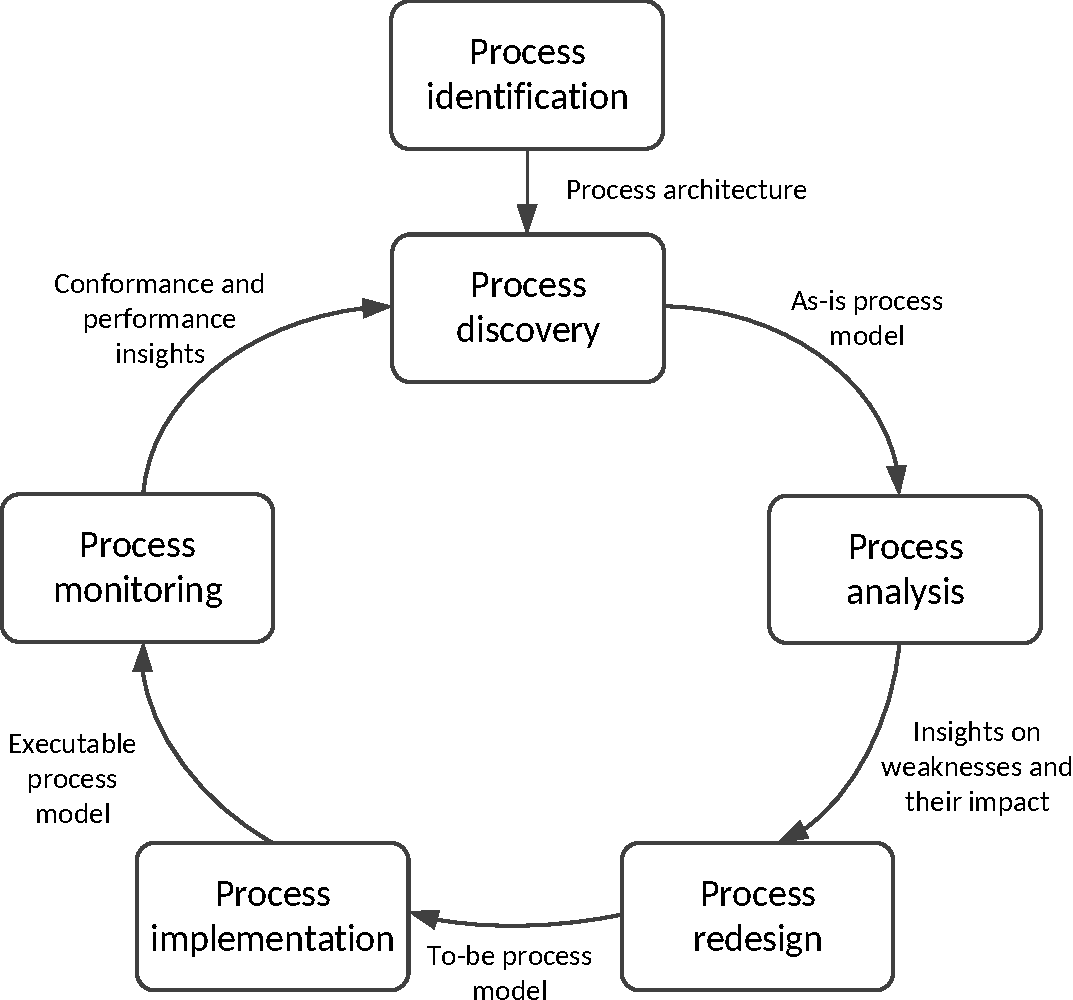
\includegraphics[width=0.8\linewidth]{figures/bpm-lifecycle}
	\caption[The BPM lifecycle]{The BPM lifecycle. Adapted from \cite[]{Dumas2018}}
	\label{fig:bpm-lifecycle}
\end{figure}

Coordination of work in business processes can be viewed from different perspectives. When analysing business processes, a good characterization can be achieved with the following four perspectives~\citep{DBLP:books/sp/Aalst16}. 
First, the \emph{control-flow perspective} aims at capturing the all the possible paths in which activities may follow one-another in a process. Second, the \emph{organizational perspective} captures which actors (e.g., people, organizational units, roles) participate in the business process and how they interact with each other. Third, the \emph{case-perspective} captures the properties of specific process instances such as the evolution of certain data-objects, originators of the case, specific values of process variables, etc. Fourth, the time-perspective captures temporal information about the process, like when and how often certain activities occurred and what was their duration.


\subsection{Process Mining}
\label{sec:process-mining}

%\subsection{Description of the field}

Process mining (\gls{pm}) is a sub-field of \gls{bpm} that emerged in the last decade, with main focus on the monitoring and discovery phases of the lifecycle. The goal is to provide fact-based insights and support process improvement. On a broader context, \gls{pm} can be considered as the missing link between traditional model-based process analysis and data driven techniques such as data mining and machine learning~\citep{DBLP:books/sp/Aalst16}. Compared to existing \gls{bi} technologies, \gls{pm} techniques go beyond the calculation of simple \glspl{kpi}. Instead, by building on model-driven approaches, they provide means to gain transparency on several aspects of the end-to-end business process. More specifically \gls{pm} techniques can infer models from event logs, which inform about the diverse aspects of a business process.
As defined in~\citep{DBLP:books/sp/Aalst16}, main \emph{perspectives}\footnote{Note that the different perspectives are partially overlapping. Yet, they are widely used in the \gls{bpm} community.} of a business process are the four. First, the \emph{time perspective} aims at analysing time and frequency of process events. Second, the \emph{case perspective} aims at identifying properties of process cases. Third, the \emph{organizational perspective} aims at analysing the event log to gain transparency on the resources involved in the process. Fourth, the \emph{control-flow perspective} aims at analysing the different variations of the process, i.e., in which order its constituting activities are carried out in real life. 

%These aspects can be, for example, related to the control flow (i.e., the various steps for used by the company for generating value), resources (i.e., handover of work among the different process participants), activities (i.e., how the work is broken down into several tasks), and data (i.e., which artifacts are produced and consumed by the process). 

There are three types of \gls{pm}, namely \begin{inparaenum}[\itshape i)]
	\item process discovery;
	\item conformance checking; and
	\item enhancement.
\end{inparaenum}
Process mining is becoming widely adopted with considerable number of algorithms from academia and several industry tools such as Celonis\footnote{\url{https://www.celonis.com}}, Disco\footnote{\url{https://fluxicon.com/disco}}, minit\footnote{\url{https://www.minit.io}}, LANA Process Mining\footnote{\url{https://lana-labs.com/en}} and more\footnote{\url{https://www.processmining-software.com/tools}}. 
%Mining algorithms are developed every year to deal to mine not only process workflow, but also other perspectives, i.e. organizational, data, etc. \Cref{fig:process-mining} illustrates process mining research and how it relates event data from real world and business process models.
This proposal focuses more on the discovery part, i.e., take an event log as an input and abstract process patterns from it. 


%\begin{description}
%	
%	\item[Process discovery.] This type of process mining is concerned with the inference of process models from event logs. Process discovery algorithms are typically unsupervised techniques that produce models in various notations such as Petri nets, \gls{bpmn}, \gls{epc}, etc. A example of a process discovery algorithm is the so-called $\alpha$-algorithm~\citep{VanderAalst2004}.
%	
%	\item[Conformance checking.] This type of process mining compares the model and the log of the same process. The goal is to verify if the reality as recorded in the event log corresponds to the plan as defined by the model. Possible deviations are quantified making it possible to obtain important cues about bad performance in case the model is prescriptive or noncompliance in case the model is normative. 
%	
%	\item[Enhancement.] This type for process mining is focused on improving the existing process model by using information from past executions recorded in the log. Differently from conformance, the goal is to go beyond measuring the misalignment but actually correcting the process model. Main types of corrections are \emph{repair}, where a process model is repaired to better explain the data from the log, and \emph{extension}, where a new information is added to the process model that is found in the log, e.g., labeling activities with the resource names, labeling sequence flows with durations, and so on.
%	
%\end{description}


\begin{figure}
	\centering
	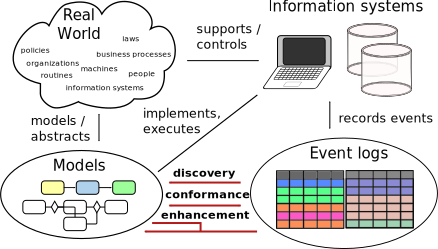
\includegraphics[width=0.9\linewidth]{figures/process-mining-big-picture}
	\caption[The process mining framework]{The process mining framework. Adapted from \citep{DBLP:books/sp/Aalst16}.}
	\label{fig:process-mining}
\end{figure}



%Nevertheless, process mining algorithms work with structured data~\citep{van2005prom, Verbeek2011}. 

%\subsection{Contribution to the research questions} 

In the context of mining the software development process, several works in the area of \gls{pm} have tackled the problem by transforming it into a \gls{pm} problem. 
%These works enrich \gls{vcs} log data with case and activity information, and then use process mining to discover a model. In this category, Kindler et al.~\citep{kindler2006activity,kindler2006incremental} can discover a Petri net from a structured and enriched version control log. This approach was further improved by Rubin et al.~\citep{rubin2007process} and a ProM\footnote{\url{http://www.promtools.org}} plug-in was provided. Poncin et al.~\citep{Poncin2011a} provide the FRASR framework for preprocessing software repositories such that they can be used in ProM. Song et al.~\citep{Song2007} help addressing the time perspective by mining a dotted chart.
Consequently, approaches have been developed to preprocess VCS data such that \gls{pm} techniques can be applied, and hence, a business process can be derived from the log data.
In this group, \citep{DBLP:conf/se/KindlerRS06,kindler2006incremental} developed an algorithm for extracting software processes that are mapped to Petri Nets. Activities, which are not explicit in the logs, are discovered from their input and output artifacts. However, strong assumptions are made on the filenames as well as on the software process lifecycle. %(always design, code, review, testres). Activities (which are not explicit in the logs, like in our case) are discovered from their input and output artifacts. Here defined as triples $<I,O,R>$ where I=input, O=Output, R=resouce who perfomed it.
\cite{rubin2007process} addressed the problem of engineering processes that are not well documented and are usually unstructured. They provided a bridge from Kindler et al.'s approach to ProM \citep{van2005prom} in order to mine different process perspectives, such as performance social network analyses. %but not from a project point of view.
\cite{rubin2014agile} applied \gls{pm} to the touristic industry and obtained user processes from web client logs pursuing the goal of improving the software system by analysing the underlying process.
\cite{DBLP:conf/csmr/PoncinSB11} developed the FRASR framework for preprocessing software repositories to transform the VCS data to logs that conform to the \gls{pm} event log meta model~\citep{van2005meta} as utilized in ProM \citep{van2005prom}.
However, these approaches disregard the single-instance nature of project-oriented business processes and treat them as procedures that can be repeated over time.
Process mining techniques are related to all the research questions of this thesis. Especially, process discovery helps with addressing \textbf{RQ4}.

%\subsection{Limitations} 
While providing interesting insights, these contributions leave out many important aspects of software development projects, such as trying to understand whether the process was done according to the organization plan. Especially, they are limited to either simply display one perspective of the process~\citep{Song2007} or transform the events from software repositories into the standard \gls{xes} format which can be mined by tools like ProM. In this case, existing methods only take into account high level information (such as the type of file) to label events accordingly. Textual information is also taken into account \citep{rubin2007process} but often limited to use of a dictionary for identifying keywords. Moreover, fine granular information on the amount of change and the comments of commit messages have not been exploited enough by existing literature.

%\todo[inline]{CHECK here! Below goes a summary that tells what process mining techniques are relevant}

%ProcesManagements mining methods work with event logs. 

To sum up, the analyses of software would benefit from a processes mining techniques, especially when it comes to uncovering behavioural patterns that are linked to the work of the developers. However, process mining techniques have not sufficiently been exploited with software development data, due to the fact that such data is not readily consumable by process mining techniques. Moreover, useful process mining techniques should provide insights that can be understood and enacted by software domain experts. Therefore, such techniques should not only look into the process but also be aware of the existing methods and performance indicators for software.  








